\section{MEASURED HVAC DIAGNOSIS STUDY}
\noindent Our principal externally grounded application is review of diagnoses from measured air-handler observations. Berkeley Lab's public collection includes both physical experiments and simulations \cite{granderson2020data}. We use only its SZCAV and SZVAV physical FLEXLAB records, pinned to Figshare version 3. The experiments imposed component faults on the air handler serving test cell X3A. They are laboratory measurements with controlled faults, not synthetic sensor observations or naturally occurring faults in occupied buildings.\draftcredit

\subsection{Evidence, Labels and Source Split}
The selected records contain 26 experimental days under constant-volume and variable-volume control. The inventory supplies the imposed condition for each day. We group stuck and leaking variants into four supported categories: normal, outdoor damper, heating valve and cooling valve. The binary fault column is cross-checked offline. Dates, filenames, fault indicators and descriptions revealing the imposed condition are withheld from model and scheduler inputs.

Each day provides three complete 60-minute windows beginning at 10:00, 12:00 and 14:00. Ten channels describe supply, outdoor, mixed and return temperatures, supply setpoints, and fan, damper and valve commands. The model receives explicitly named means, minima, maxima and changes from first to last reading. Fahrenheit units, fractional commands and recording hours are retained. Commands are not assumed to measure actual component position. No later observations enter a window's evidence. Figure~\ref{fig:measured} connects a recorded example to its generated diagnosis.

The first chronological day of each mode and category is development, giving eight days and 24 windows. The remaining 18 days and 54 windows form the frozen evaluation. Adjacent windows never cross the split. All included days are selected from source records before evaluation generation, without filtering on errors or policy performance. A standardized nearest-centroid classifier fits its normalization and class centers using development data alone and uses the same statistics, control mode and hour as the model.

\begin{figure*}[t]
\centering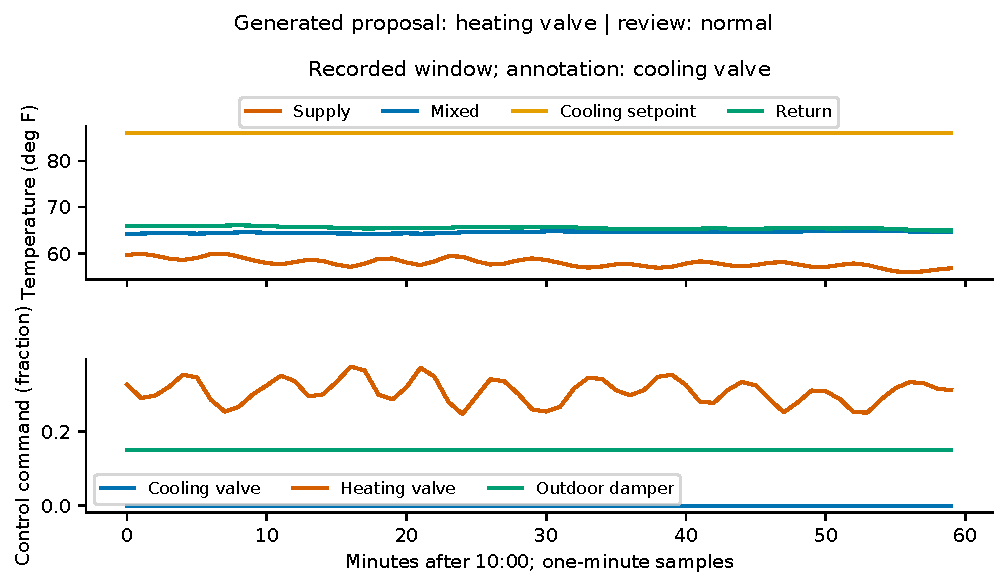
\includegraphics[width=0.84\textwidth]{../artifacts/stage7_empirical/figures/measured_example.pdf}
\caption{Measured temperatures and control commands from the first source-order evaluation window. The cooling-valve annotation comes from the experiment inventory and is shown only for analysis. The agent receives window summaries, without that annotation or source date. Both its generated heating-valve proposal and the model review's normal diagnosis are wrong. Recorded cooling despite a zero cooling-valve command illustrates information that the weak proposer failed to use reliably.}
\label{fig:measured}
\end{figure*}

\subsection{Fallible Review and Expected Benefit}
The pinned Qwen model generates one diagnosis and then a separately prompted review of that diagnosis and the same permitted observations. The review may preserve the category, change it or abstain. These responses are correlated same-model judgments, not independent experts. An initial development pilot exposed ambiguous numerical arrays and frequent abstention. One declared revision names every statistic and requests the most likely supported category. All failed pilot outcomes remain saved. No further prompt change follows evaluation.

For an error indicator $E_i$ before review and $E_i^R$ after review, define the conditional expected accuracy gain
\begin{equation}
 g_i=\Pr(E_i=1,E_i^R=0\mid x_i)-\Pr(E_i=0,E_i^R=1\mid x_i).
\end{equation}
Here $x_i$ is public proposal information. A harmful abstention counts as an unresolved task. The modeled benefit of timely review is $w_i g_i$, rather than $w_i p_i$. We estimate risk by $(e+1)/(n+2)$ and signed gain by $(c-h)/(n+2)$ from development errors $e$, corrections $c$ and harms $h$. Proposed-category bins with fewer than six examples use the pooled estimate. This is a transparent small-data shrinkage rule, not a well-established reviewer model.

The revised development set has six correct proposals, one correction and one harmful review. Pooled gain is zero, and the populated heating-proposal bin has negative gain. Thus positive-benefit eligibility declines every review in the primary condition. This mathematical consequence is frozen before evaluation. A secondary risk-only condition deliberately ignores reviewer harm while applying the same saved responses. An ideal condition returns the annotated category only when selected review completes. It bounds reviewer effectiveness, without giving hidden labels to scheduling.

\subsection{Constructed Oversight Dynamics}
The three windows become retrospective diagnosis tickets after 14:59, and all are released at abstract tick zero. They describe the same equipment and imposed condition, not three independent machines. The experiment models allocation across competing diagnostic outputs, not physical repair. Cutoffs 2, 4 and 6 and dimensionless error weights 4, 8 and 12 are independently permuted by a public run seed. An incorrect or unresolved ticket incurs its weight at cutoff. A timely completed review can change the diagnosis before that point. It cannot undo a past consequence or establish subsequent repair success.

We freeze one or two reviewer slots, service durations of one, two or three ticks, and a uniform-weight sensitivity with weight eight. Equal-time completion is timely. Search enumerates the current queue and assigns proposed reviews to the next available slot. Measured GPU latency is recorded separately from these assumed service times. All six policies reuse identical saved proposals and review responses. This yields 3,888 paired policy replays without additional generations.

The primary contrast is search minus greedy loss with signed-gain model review, one slot, two-tick service and heterogeneous weights. We resample whole experimental days 2,000 times with seed 20260917, stratifying by control mode and keeping all matched conditions together. Eighteen day blocks on one piece of equipment support conditional within-facility summaries. With one physical unit there is no stable equipment-level interval. Day-block exchangeability is unverified, so the intervals are conditional resampling summaries. The 54 windows are not 54 independent cases.

\subsection{Diagnostic and Allocation Results}
The proposer correctly labels 19 of 54 windows (35.2\%), versus 27 (50.0\%) for the conventional classifier. It proposes a heating-valve fault on 51 windows, correctly identifying all 18 heating cases but none of the 15 cooling or 12 damper cases. The conventional baseline identifies 14 heating, seven damper and six normal windows, but also misses every cooling case. The task remains difficult for both methods. Day-level imposed-condition labels do not guarantee that each selected window excites a detectable fault symptom. Low accuracy therefore reflects the full representation and diagnosis task, not an isolated measure of reasoning skill. These results establish a diagnosis bottleneck rather than a reliable deployed detector.

Across saved review pairs, review corrects one of 35 wrong proposals and leaves 34 unresolved. It preserves 13 of 19 correct proposals, changes five to a wrong category and abstains on one. Five review responses abstain in total. There are no malformed proposals, malformed reviews or failed generation attempts in the final evaluation. Review-everything accuracy is 14/54, below initial accuracy. Frozen risk has Brier score 0.2305 and AUROC 0.5023. Sparse, nearly tied risks provide little discrimination.

All primary policies decline review and have mean loss 15.333 with 19 correct diagnoses. Search minus greedy is exactly zero on all 18 day blocks. The degenerate paired interval describes a shared frozen admission rule, not evidence that scheduling policies are equivalent. Ignoring reviewer harm produces search and greedy loss 18.000, although search performs 54 reviews versus 39. Their sequences differ on 15 days with no loss difference. Risk-only search is worse than no review by 2.667 points, with interval [0.217,5.778].

Under ideal review, search attains zero loss versus greedy's 3.333, a paired difference of $-3.333$ [$-4.889,-1.778$], with ten day wins, eight ties and no losses. EDF also attains zero and chooses the same sequence as search. With three simultaneous equal-duration requests and cutoffs 2, 4 and 6, earliest-deadline ordering can fit every two-tick review. This structural explanation limits the interpretation of the ideal-reference advantage. Figure~\ref{fig:hvacpolicies} shows correctness alongside modeled loss. Capacity sensitivity, all day differences and first-qualifying timelines are in the supplement. No measured equipment damage, energy saving or human-review effectiveness follows from these results.

\begin{figure*}[t]
\centering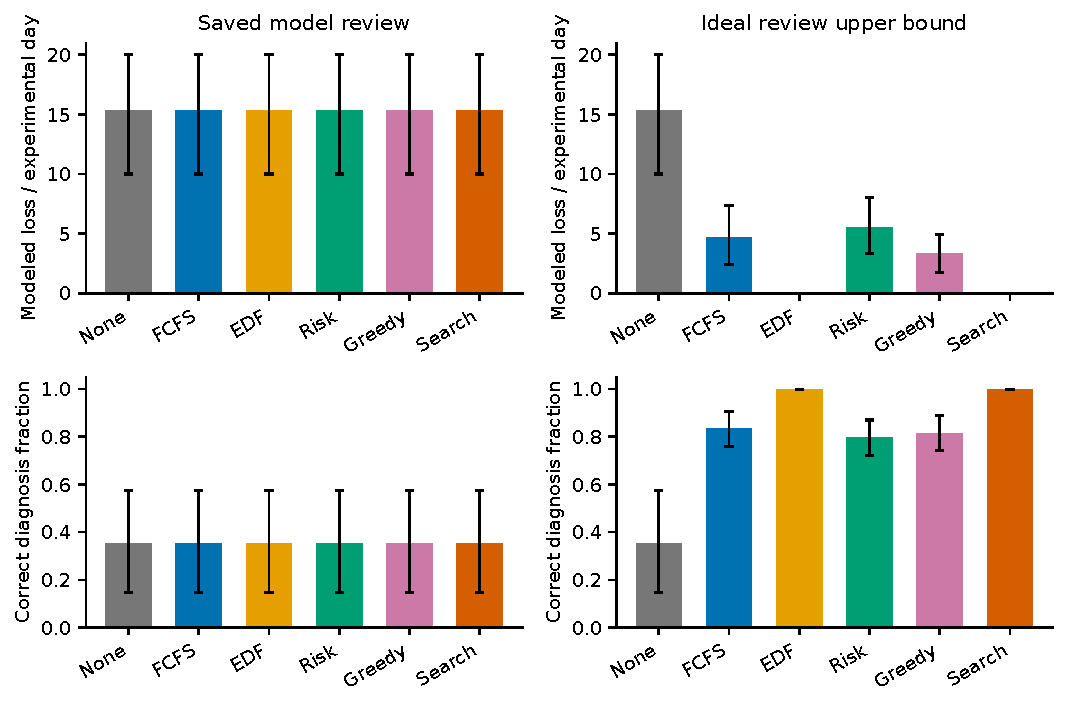
\includegraphics[width=0.96\textwidth]{../artifacts/stage7_empirical/figures/policy_performance.pdf}
\caption{Externally annotated diagnosis correctness and simulated weighted loss, one reviewer and two-tick service. The left condition uses development-fitted signed model-review benefit and admits no reviews. The right assumes ideal completed review. Proposals are generated from measured windows; loss weights and scheduling dynamics are constructed. Bars show 95\% day-block bootstrap intervals conditional on one facility, with all paired windows and conditions retained.}
\label{fig:hvacpolicies}
\end{figure*}
